\setcounter{framenumber}{24}
\begin{frame}
	\maketitle
\end{frame}

\begin{frame}{Overview}
\tableofcontents
\end{frame}

\section{Rehash}
\begin{frame}{Rehash}

\begin{itemize}

	\item \alert{Read the syllabus!}
	
	\item Logic is the study of valid reasoning.
	
	\item An inference is valid iff in every situation where the premises are true, the conclusion is true.
	
	\item \alert{We develop a \emph{mathematical} account of validity.}
	
	\item We restrict ourselves to classical propositional and first-order logic.
	
	\item A logic is decidable iff there's an algorithm for determining validity. First-order logic is \emph{not} decidable.

\end{itemize}

\end{frame}

\section{2. A Mathematics Primer for Aspiring Logicians}
\begin{frame}{2.0 Literature Recommendation}

	\begin{center}
		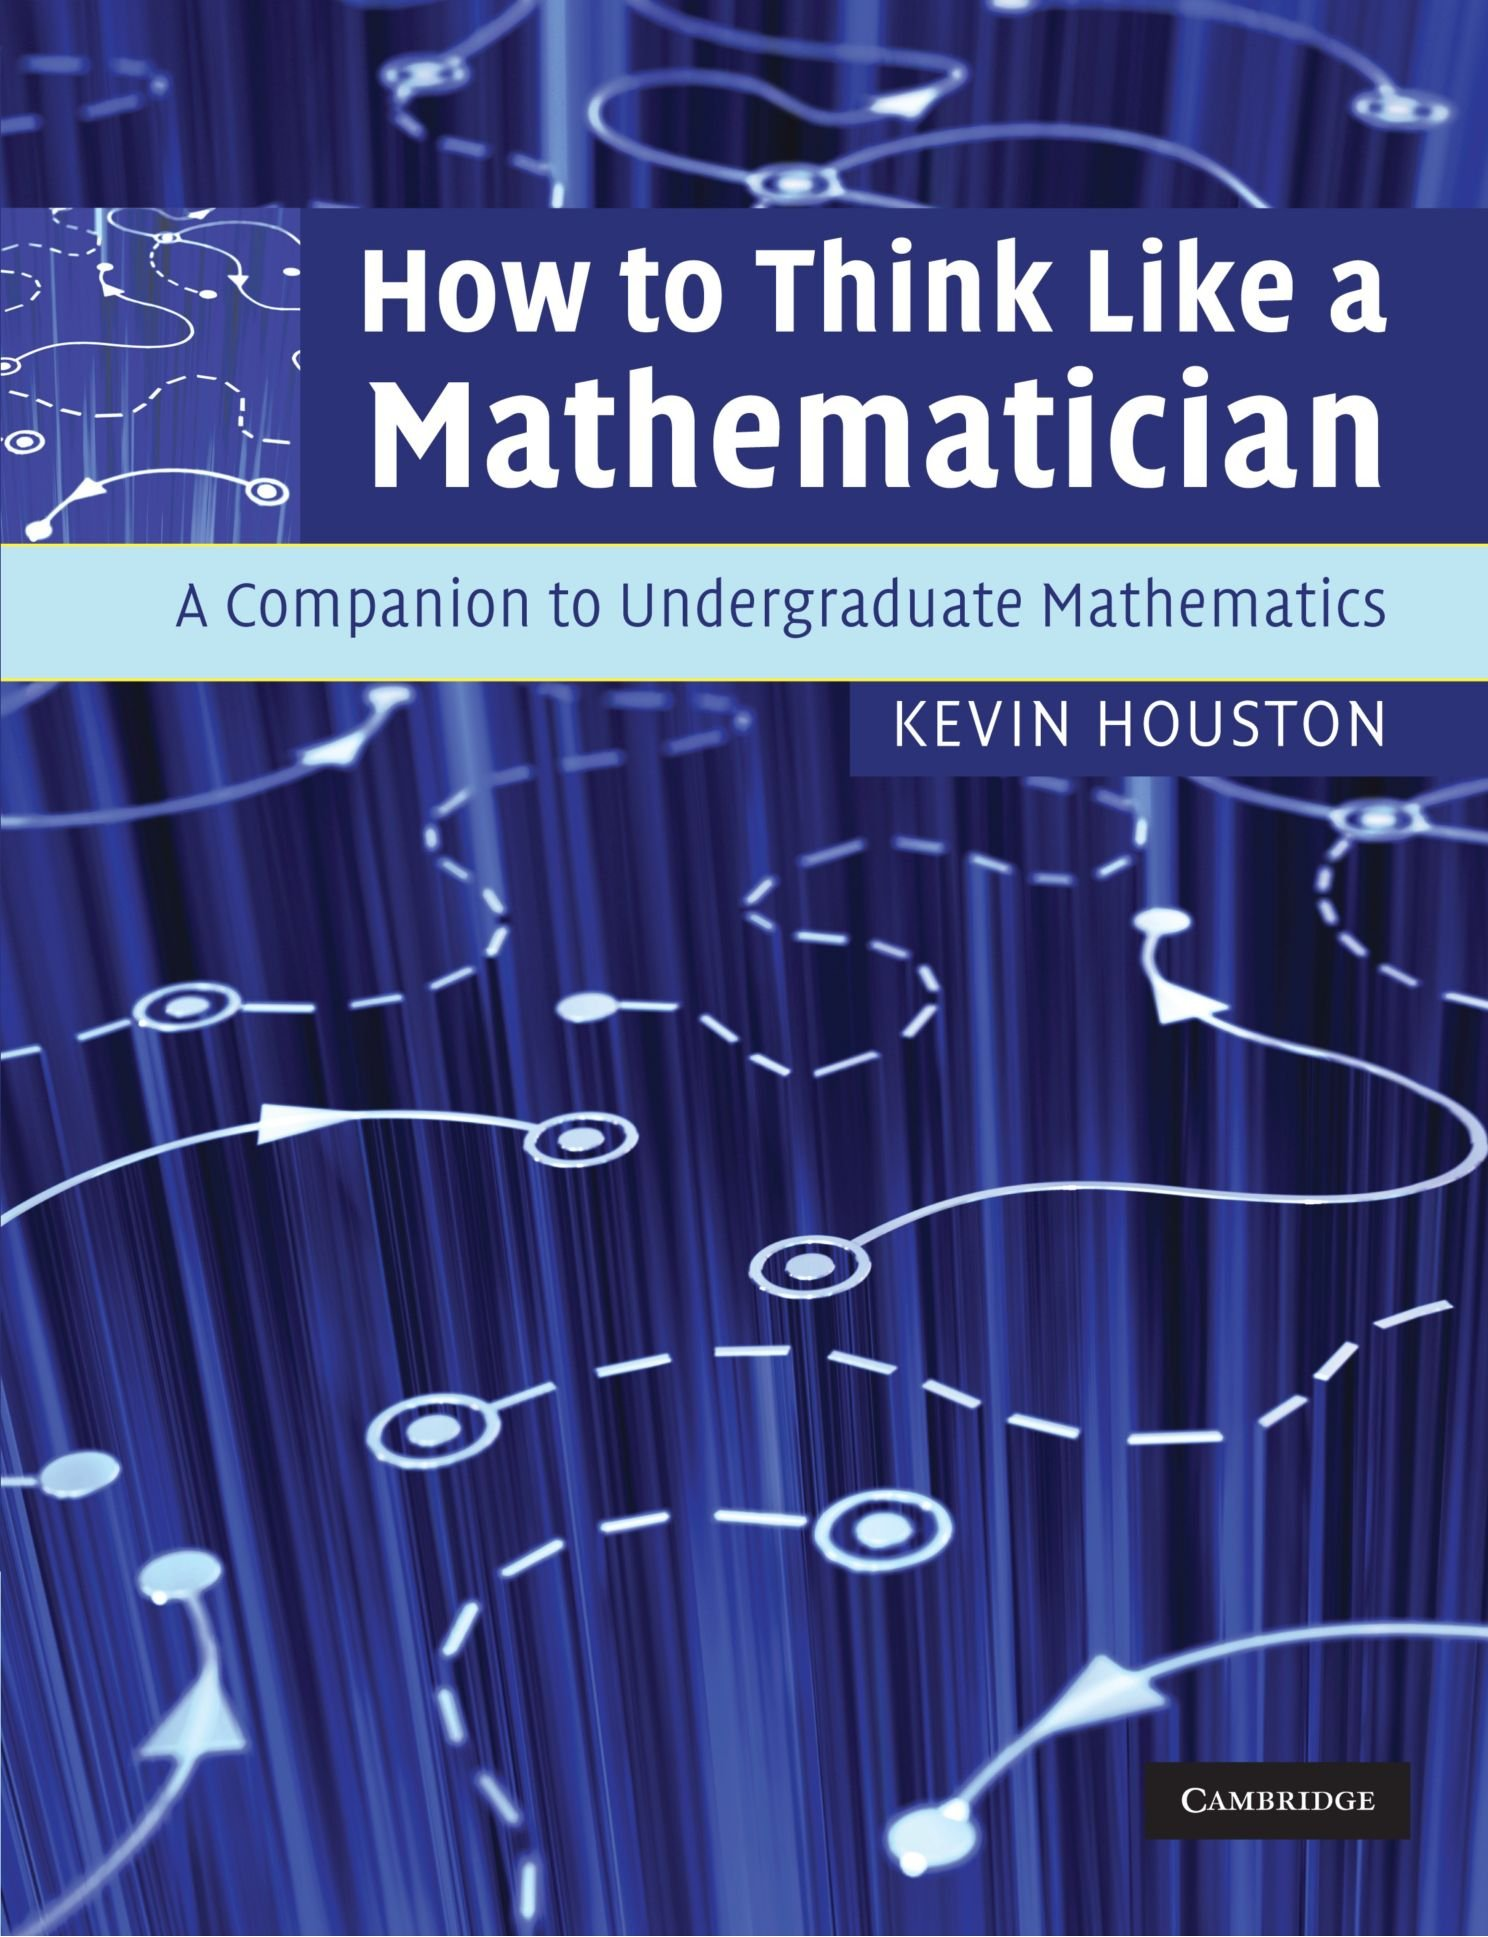
\includegraphics[width=15ex]{houston-httlam}
	\end{center}

Houston, Kevin. 2009. \emph{How to Think Like a Mathematician.} Cambridge, UK: CUP. (HTTLAM)

\begin{itemize}

	\item \emph{Not} a mandatory reading!
	
	\item I will lecture on some ideas from this book.

	\item The book has a webpage:

	\begin{center}
	\url{http://www.kevinhouston.net/httlam.html}
	\end{center}
	
\end{itemize}

\end{frame}


\subsection{2.1 Logic and Mathematics}
\begin{frame}{2.1 Logic and Mathematics}

	\begin{itemize}

		\item (2.1.1) Logic today is highly mathematized.
		
		\item (2.1.2) We distinguish between:
		
			\begin{itemize}
			
				\item \emph{Mathemateze} --- the language of mathematics (\S2.2)
				
				\item \emph{Mathodology} --- the method of mathematics (\S2.3)
			
			\end{itemize}
			
			\item You have to \emph{learn} to talk and think like a mathematician.
			

			%\item (2.1.3) We use logic and mathematics to study logic. This is just like studying English grammar in English.
	
	\end{itemize}
	
	\begin{center}
		\begin{tabular}{c}
		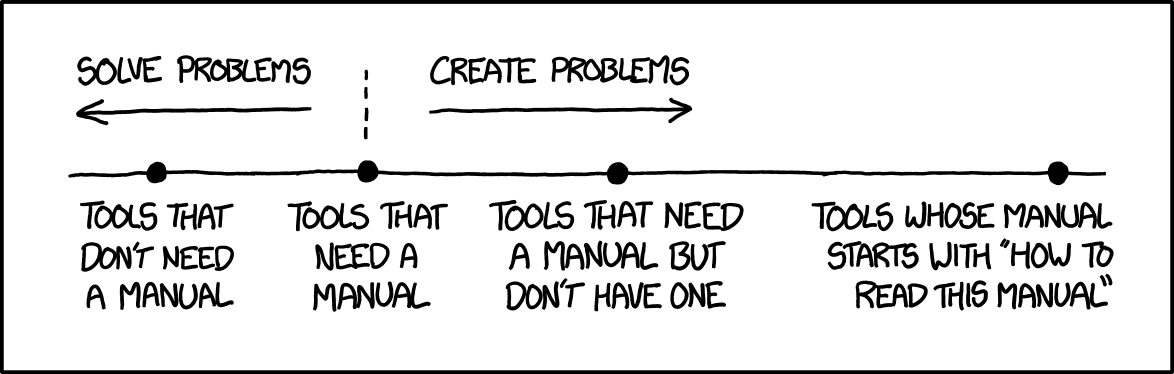
\includegraphics[width=40ex]{xkcd-manuals}\\[-1ex]
		{\tiny \textcopyright~\url{https://xkcd.com/1343/}, CC BY-NC 2.5}
		\end{tabular}
		\end{center}
	
\end{frame}

\subsection{2.1 Mathemateze}
\begin{frame}{2.1 Mathemateze}
		
	

A systematic method for reading math (HTTLAM, p. 16):
		
			\begin{enumerate}[(i)]
			
				\item Skim 
				
				\begin{itemize}
				
					\item Identify what's important
				
				\end{itemize}
				
				\item Ask questions
			
				\item Read carefully
				
					\begin{itemize}
					
						\item Stop to review
						
						\item Read statements first, proofs later
											
					\end{itemize}
				
				\item Be active
				
					\begin{itemize}
						
						\item Check the text 

						\item Do exercises and problems
					
					\end{itemize}
				
				\item Reflect
				
					\begin{itemize}
						
						\item Write a summary
						
						\item Move on
						
						\item Return
					
					\end{itemize}
			
			\end{enumerate}
	
		
\end{frame}

\begin{frame}{Variables}

	\[(a+b)^2=a^2+2ab+b^2\]
	
	\begin{itemize}
	
		\item (2.2.3) Variables stand for arbitrary but fixed objects.
		
		\item (2.2.4) Always declare your variables:
		
			\begin{itemize} 
			
				\item Let $n$ be a natural number. 
							
				\item For $n$ a natural number, \dots.
				
				\item Consider a natural number $n$.
				
				\item Suppose that $n$ is a natural number. 
			
			\end{itemize}
		
		\item (2.2.6--7) Variables allow us to make general claims:
		
			\begin{itemize}
			
				\item For all natural numbers $n$ and $m$, it holds that $n+m=m+n$.
				
				\item There exists a number $n$, such that $n$ is the smallest prime bigger than $436\cdot 10^99$.
			
			\end{itemize}
			
		\item (2.2.10) Variables are bound by context.
	
	\end{itemize}

\end{frame}

\begin{frame}{Indices}

Natural numbers are often used to \emph{count} objects:

	\begin{itemize}
	
		\item Suppose that there are $n$ apples, $a_1, \mathellipsis, a_n$.
		
		\item Let $a_i$ be one of those apples (for $1\leq i\leq n$).
		
		\item The variable $i$ ranges over the numbers from one to ten.
		
		\item For each $i$, the variable $a_i$ ranges over the apples.
	
	\end{itemize}
	
	\begin{center}
		\begin{tabular}{c}
		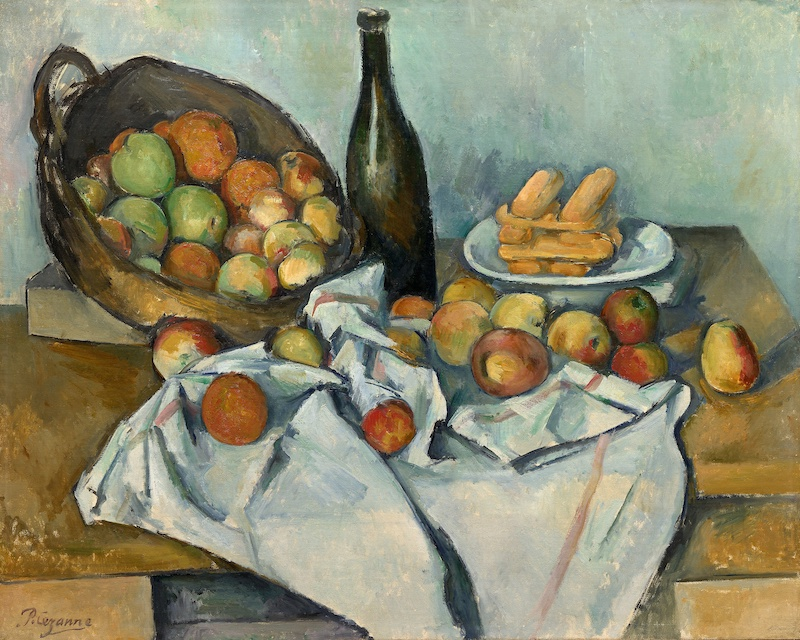
\includegraphics[width=30ex]{cezanne-apples}\\[-1ex]
		{\tiny $\not\hspace{-1ex}\textcopyright$ C\'ezanne, \emph{The Basket of Apples}, work in public domain}
		\end{tabular}
		\end{center}

\end{frame}

\begin{frame}{Standard Variables (2.2.5)}

Some variables with implicit declarations:

	\begin{center}
	\begin{tabular}{l | l}
			Object & Variable\\\hline
			
			unspecified & $x,y,z,\mathellipsis$\\
			
					& sometimes: $a,b,c, \mathellipsis$\\
			
			natural numbers & $n,m,l,\mathellipsis$\\
			
			indices & $i,j,\mathellipsis$ \\
			
			sets of indices & $I,J,\mathellipsis$\\
			
			functions & $f,g,h,\mathellipsis$\\
			
					& also: $\lambda, \sigma,\tau,\mathellipsis$\\
			
			sets & $X,Y,Z,\mathellipsis$ \\
			
			conditions & $\Phi,\Psi,\mathellipsis$\\
			
			formulas	 & $\phi,\psi,\theta,\mathellipsis$\\
			
					& also: $A,B,C, \mathellipsis$\\
					
			propositions & $p,q,r, \mathellipsis$\\
					& also: $P,Q,R,\mathellipsis$
			
			\end{tabular}
		\end{center}

But just to be sure (at least for now) \emph{always} declare your variables!		
		
\end{frame}

\begin{frame}{Constants}

\[e^{i\pi}+1=0\]
	
	\begin{itemize}
	
		\item (2.2.11) Constants stand for distinguished mathematical objects.
		
		\item There are constants for all sorts of objects:
		
			\begin{center}
				\begin{tabular}{c | c}
				Objects & Constants\\\hline
				Natural numbers & $0,1,2,\mathellipsis$\\
				Integers & $-1, -2, -3, \mathellipsis$\\
				Rational numbers & $\frac{1}{2}, \frac{2}{3}, \frac{4}{5},\mathellipsis$\\
				Real numbers & $\pi,\sqrt{2}, e,\mathellipsis$\\
				Complex numbers & $i, -i, 1+3i,\mathellipsis$\\
				Functions & $+, \cdot, \sin,\cos, \exp,\mathellipsis$\\
				Relations & $\leq, <, |, \bot,\mathellipsis$'\\
				Sets & $\mathbb{N}, \mathbb{Z}, \mathbb{Q}, \mathbb{R},\mathbb{C}, C^\infty(\mathbb{R}),\mathellipsis$ 
				\end{tabular}
			\end{center}
			
		\item (2.2.12) Sometimes, we use \emph{temporary} constants: $a,b,c,\mathellipsis.$
		
		\item But they're really just variables.
	
	\end{itemize}

\end{frame}

\begin{frame}{Mathematical Statements (HTTLAM, \S6)}

	\begin{itemize}
	
		\item (Def. 6.1) A \emph{(mathematical) statement} is a sentence (in mathemateze) that is either true or false --- but not both.
		
		\item \emph{Examples}.
		
			\begin{itemize}
			
				\item $5+7=12$
				
				\item $0=1$
				
				\item There are no natural numbers $n,m$, such that $(\frac{n}{m})^2=2$
				
				
				\item There exists a natural number $n$ such that for all other natural numbers $m$, we have $m\leq n$.
			
			\end{itemize}
			
			\item For $A,B$ statements:
			
				\begin{itemize}
				
					\item the \emph{negation} of $A$ is  `not-$A$'
					
					\item the \emph{conjunction} of $A$ and $B$ is `$A$ and $B$'
					
					\item the \emph{disjunction} of $A$ and $B$ is `$A$ or $B$'
					
					\item the \emph{conditional} of $A$ and $B$ is `if $A$, then $B$'
				
				\end{itemize}
				
			\item De Morgan Laws:
			
				\begin{itemize}
				
					\item not-($A$ and $B$) is the same as not-$A$ or not-$B$
					\item not-($A$ or $B$) is the same as not-$A$ and not-$B$
				
				\end{itemize}
	
	\end{itemize}


\end{frame}

\begin{frame}{If and Only If (Iff) --- Equivalence}

\begin{itemize}

	\item (2.2.13) To say that $A$ iff $B$ is to say that $A$ and $B$ are equivalent:
	
	\begin{itemize}
	
		\item If $A$ and $B$ are equivalent, then they can be replaced for each other.
		
		\item $A$ iff $B$ is the same as if $A$, then $B$ and if $B$, then $A$
	
	\end{itemize}
	
	\item \emph{Examples}:
	
	\begin{itemize}
	
		\item A number $n$ is smaller than a number $m$ iff there exists a number $k$ such that $n+k=m$.
		
		\item An inference is valid iff in every situation where the premises are true, so is the conclusion.
		
		\item A number $n$ is even iff $n+1$ is odd.
	
	\end{itemize}
	
		\begin{center}
		\begin{tabular}{c}
		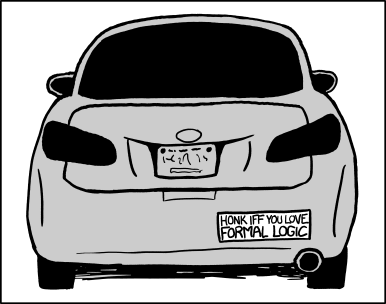
\includegraphics[width=20ex]{xkcd-iff}\\[-1ex]
		{\tiny \textcopyright~\url{https://xkcd.com/1033/}, CC BY-NC 2.5}
		\end{tabular}
		\end{center}

\end{itemize}

\end{frame}

\begin{frame}{Definitions}

	\begin{itemize}
		
		\item \emph{Examples} (HTTLAM \S15, p.~103--4):
	
	\begin{enumerate}[(i)]
	
		\item An integer is \emph{even} if it is the product of 2 and another integer.
		
		\item An integer is \emph{odd} if it is not even.
		
		\item We call a set $X$ with a \emph{finite number} of elements a finite set.
		
		\item If a natural number greater than 1 is divisible only by 1 and itself, then it is called \emph{prime}.
		
		\item A prime number $p$ is called a \emph{twin prime} if $p-2$ or $p+2$ is prime.
		
		\item A positive integer $n$ is a \emph{square number} if $n= x^2$ for some integer $x$.
		
		\item A natural number is called \emph{squarey} if its digits are the last digits of its square.
		
		\item A prime number is called \emph{squarey-twinney} if it is a twin prime and is squarey.
	
	\end{enumerate}
	
	\item \emph{Further examples}:
	
		\begin{enumerate}[(i)]
		\setcounter{enumi}{8}
		
			\item The number $0$ is defined as the smallest natural number.
		
			\item The number $\pi$ is defined as $\int_{-1}^{1}\frac{1}{\sqrt{1-x^2}}dx$
			
			\item The exponentiation function $\exp(x)$ is defined as $\sum_{n=0}^\infty\frac{x^n}{n!}$
		
		\end{enumerate}
	
	\end{itemize}

\end{frame}

\begin{frame}{Two Kinds of Definitions}


	\begin{itemize}

		\item The point of a definition is to give the meaning of a mathematical expression.
		
		\item There are two kinds of mathematical definitions:
		
			\begin{itemize}
			
				\item definitions of \emph{objects} (numbers, functions, sets, \dots)
				
				\item definitions of \emph{properties} and \emph{relations} (being prime, smaller than, \dots)
			
			\end{itemize}
			
	\end{itemize}
	
	\begin{center}
		\begin{tabular}{c}
		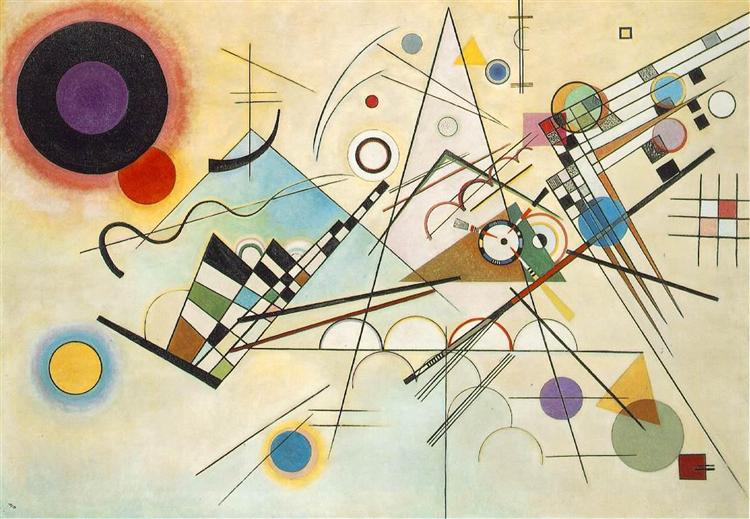
\includegraphics[width=40ex]{kandinsky-komp8}\\[-1ex]
		{\tiny $\not\hspace{-1ex}\textcopyright$ Kandinsky, \emph{Komposition 8}, work in public domain}
		\end{tabular}
		\end{center}

\end{frame}

\begin{frame}{Definitions of Objects}

	\begin{itemize}
	
		\item (2.2.17--18) A mathematical object is defined by giving a list of properties that this and only this object has.
		
		\begin{itemize}

		\item \emph{Example.} We define $\sqrt{2}$ as the positive real $x$ such that $x^2=2$.
		
		\end{itemize}
		
		\item In order for the definition of an object to be successful we need to show:
		
		\begin{description}
		
			\item[Existence.] There exists an object that satisfies the properties.
						
			\item[Uniqueness.] There can only be one object that satisfies the properties.
		
		\end{description}
		
		\item So:
		
			\begin{itemize}
			
				\item ``Let $\omega$ be the biggest natural number'' is unsuccessful (existence condition violated).
				
				\item ``$\sqrt{2}$ is the real $x$ s.t. $x^2=2$'' is unsuccessful (uniqueness condition violated).
			
			\end{itemize}
			
		\item We'll discuss definitions of functions and sets next lecture.
	
	\end{itemize}

\end{frame}

\begin{frame}{Definitions of Properties and Relations}

	\begin{itemize}
	
		\item (2.2.19) A property is defined by listing the conditions for an object to have the property.
		
		\begin{itemize}
		
			\item \emph{Example}. An integer number $n$ is even iff there exists an integer $k$ such that $n=2\cdot k$.
	
		\end{itemize}
		
		\item (2.2.24) A relation is defined by listing the conditions for objects to stand in the relation.
		
		\begin{itemize}
		
			\item \emph{Example}. A natural number $n$ divides another natural number $m$, $n|m$, iff there exists a natural number $k$ such that $n\cdot k=m$.
	
		\end{itemize}
				
		\item Definitions are iff-statements:
		
		\begin{itemize}
		
			\item \emph{Necessary condition}: A condition without which something can't be (`only if').
			
			\item \emph{Sufficient condition}: A condition that guarantees that something is the case (`if').
		
		\end{itemize}
		
		\item For a definition to be successful, it mustn't be \emph{circular}:
		
		\begin{itemize}
		
			\item ``$n$ is even iff there are even numbers $k,l$ such that $n=k\cdot l$'' is unsuccessful because circular 
		
		\end{itemize}
	
	\end{itemize}

\end{frame}



\begin{frame}{How to Understand a Definition (2.2.26)}

\begin{itemize}

	\item \emph{How to read a definition} (HTTLAM \S15, p.~105--7):
	
		\begin{itemize}
		
			\item \emph{Observe!} (What are the conditions?)
			
			\item \emph{What are we dealing with?} (Definition of an object, definition of a property/relation, \dots)
			
			\item \emph{Think through examples!}
			
				\begin{itemize}
				
					\item Standard examples ($3,5,$ and $7$ are prime)
					
					\item Trivial examples ($0$ is even)
					
					\item Extreme examples ($2$ is a prime)
					
					\item Counter-examples ($1$ isn't a prime)
				
				\end{itemize}
				
			\item \emph{Create new objects from old ones!}
		
			\begin{itemize}
			
				\item If $n$ is prime, is $n+2$ prime? (Yes for $(5,7)$, no for $(7,9)$!)
			
			\end{itemize}
		
		
		\end{itemize}

\item I'd like to add:
		
		\begin{itemize}
		
			\item \emph{Think of (non-)equivalent definitions!}
			
			\begin{itemize}
			
				\item Can we define primes in another way?
				
				\item  Is there another definition of $\pi$?			
			\end{itemize}
			
			\item \emph{Check properties!}
			
			\begin{itemize}
			
				\item Is $\pi$ rational?
				
				\item  Is $0$ even?	
						
			\end{itemize}
		
		\end{itemize}
		
\end{itemize}

\end{frame}

\begin{frame}{Writing Mathematics --- Formal vs. Informal}

	\begin{itemize}
	
		\item (2.2.29) There is a trade-off between precision (formal) and understandability (informal).
		
		\item Use this to your advantage: $[\not\hspace{-.5ex}x]$ exercises!
		
		\item \emph{Writing advice} (HTTLAM \S3--4):
		
		\begin{itemize}
		
			\item Write in simple, punctuated sentences.
			\item Keep it simple.
			\item Explain your actions and assertions.
			\item Say what you mean.
			\item Words $>$ Symbols.
			\item No arrows.
			\item Proofread.
			\item Don't begin sentences with symbols.
			\item Don't (over)use it.
			
		\end{itemize}

	
	\end{itemize}

\end{frame}

\subsection{2.3 Mathodology}

\begin{frame}{2.3 Mathodology --- The Art of Proving Things}

	\begin{itemize}
	
		\item (2.3.1) A mathematical proof is a rigorous, step-by-step argument which establishes the truth of a mathematical statement.
	
		\item (2.3.3) The ideal of mathematical proof is \emph{axiomatic} proof.
		
		\begin{itemize}
		
			\item An \emph{axiom} is a basic principle of mathematics, which is assumed to be true.
			
			\item An axiomatic proof is one with only axioms and definitions and each step a valid inference.
			
			\item Axiomatic proofs are long and hard to read.
		
		\end{itemize}
		
		\item (2.3.4) Instead, we practice \emph{informal rigor}: we aim to convince the reader that a purely axiomatic proof exists.
	
	\end{itemize}
	
	
	\begin{center}
		\begin{tabular}{c}
		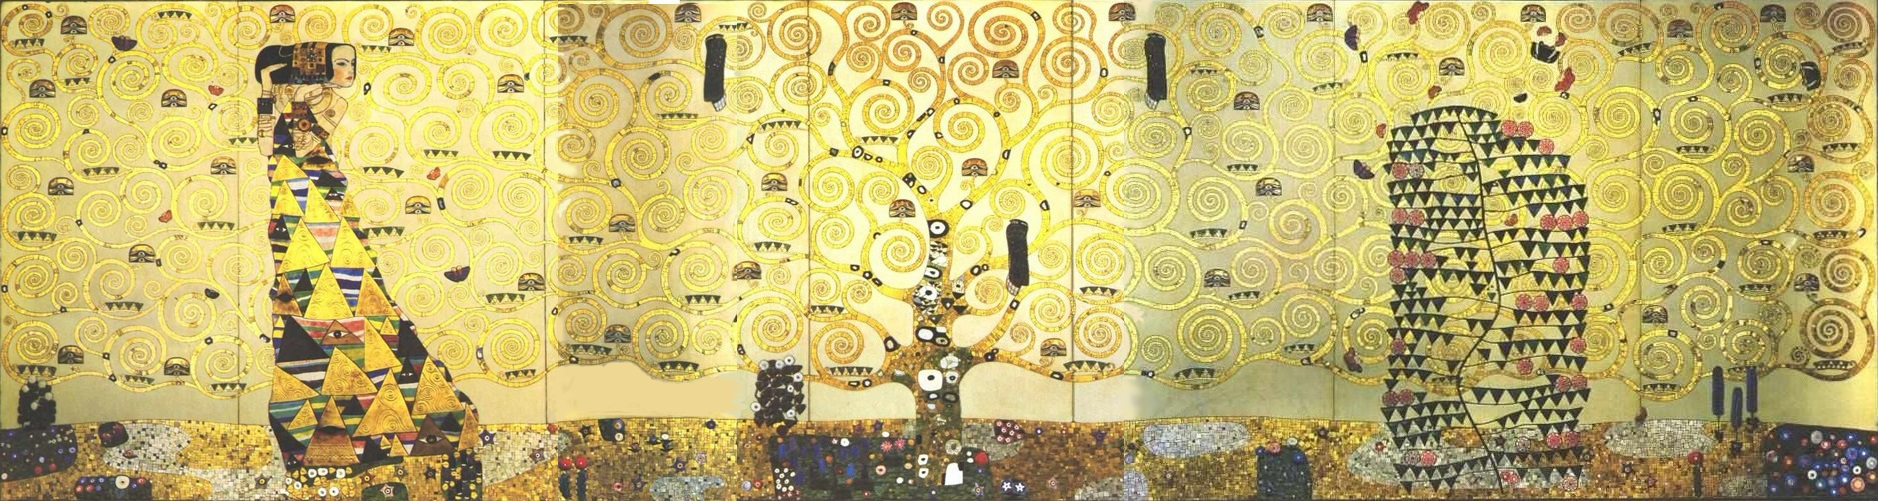
\includegraphics[width=60ex]{klimt-tree}\\[-1ex]
		{\tiny $\not\hspace{-1ex}\textcopyright$ Klimt, \emph{Stoclet-Fries}, work in public domain}
		\end{tabular}
		\end{center}


\end{frame}

\begin{frame}{Some Terminology}

	\begin{center}
	
		\begin{tabular}{c  p{.75\linewidth}}
			
			\textbf{Lemma.} & An auxilliary claim, established in order to prove a more important proposition or theorem.\\
			
			\textbf{Proposition.} & A run-of-the-mill, ordinary mathematical fact.\\
			
			\textbf{Theorem.} & An important mathematical fact (also used generically for mathematical facts)\\
			
			\textbf{Corollary.} & A simple consequence of a previously established lemma, proposition, or theorem.\\[2ex]
			
	\hline\\[2ex]
	
	
\textbf{Conjecture.} & A putative mathematical fact.	
	
	
		\end{tabular}
	\end{center}


\end{frame}

\begin{frame}{De-mystifying Mathematical Proofs}

	\begin{center}
		\begin{tabular}{c}
		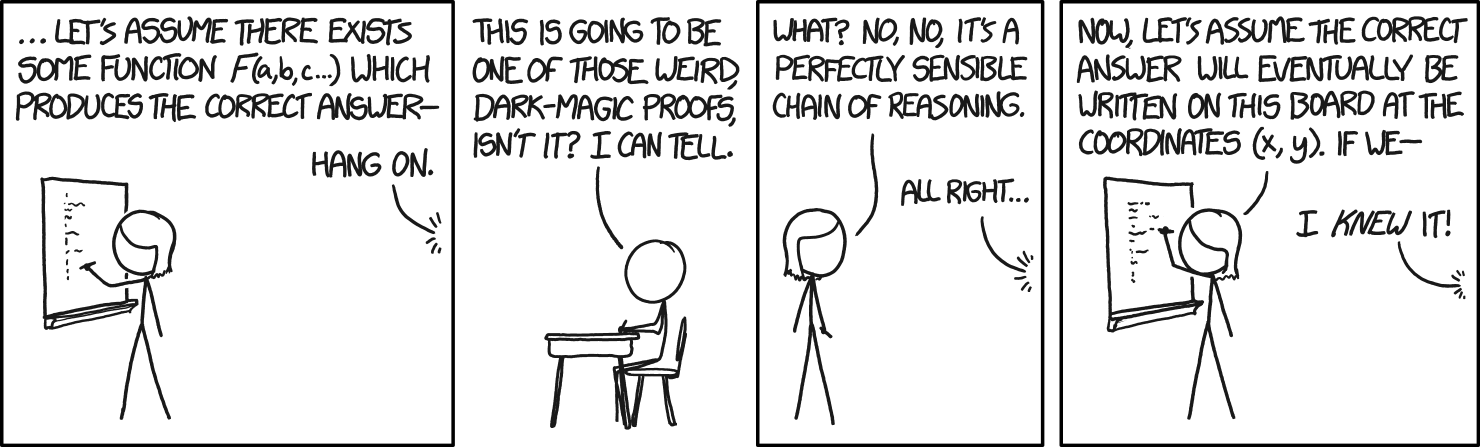
\includegraphics[width=60ex]{xkcd-proofs}\\[-1ex]
		{\tiny \textcopyright~\url{https://xkcd.com/1724/}, CC BY-NC 2.5}
		\end{tabular}
		\end{center}
		
	How \emph{do} you prove something?

\end{frame}

\begin{frame}{Problem Solving --- Proving is Problem Solving!}

\begin{center}
		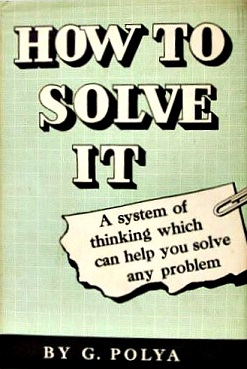
\includegraphics[width=15ex]{polya-problem}\\
		Polya, Georg. 1945. \emph{How To Solve It.} 1$^\text{st}$ Edition. Princeton, NJ: Princeto Univeristy Press. (Many, many reprints, 2$^\text{nd}$ edition, \dots.)
		\end{center}

	\begin{itemize}
		
		\item \emph{Polya's Four-Step Plan} (HTTLAM, \S5):
		
			\begin{enumerate}[(i)]
			
				\item \emph{Understand the problem}
				
					
				
				\item \emph{Devise a plan}
				
					
				
				\item \emph{Execute the plan}
				
				
				
				\item \emph{Look back}
			
			\end{enumerate}

	\end{itemize}
	
\end{frame}

\begin{frame}{Understand the Problem}

		\begin{itemize}
					
						\item Understand the words and symbols
						
						\item Guess
						
						\item What do you know already?
						
						\item Work backwards and forwards
						
						\item Look at examples (initial, special, and concrete cases)
						
						\item Work with a concrete case
						
						\item Think about a similar problem
						
						\item Draw a picture
						
						\item Find an equivalent problem
						
						\item Solve an easier problem (e.g. special case case)
						
						\item Rewrite (symbols \reflectbox{$\leadsto$} $\leadsto$ words)
					
					\end{itemize}

\end{frame}

\begin{frame}{Devise a Plan, Execute, and Look Back}


	\begin{itemize}
	
		\item In order to devise a plan:

		\begin{itemize}
					
						\item Break the problem into pieces
						
						\item Find the right level (applying theorems or definitions)
						
						\item Give things names
						
						\item Systematically choose a method (covered below)
						
					\end{itemize}

		\item While executing:

				\begin{itemize}
					
						\item Check each step! --- Don't use intuition
					
					\end{itemize}
					
					
		\item Afterwards, look back
					
					
					
					\begin{itemize}
					
						\item Check the answer, can it be improved?
						
						\item Is there another proof?
					
					\end{itemize}
					
		\end{itemize}
		
		\begin{center}
		\begin{tabular}{c}
		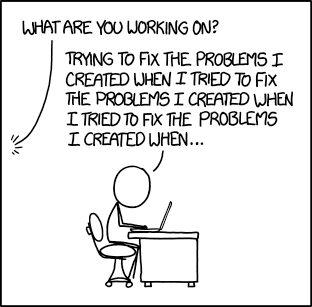
\includegraphics[width=15ex]{xkcd-fixing}\\[-1ex]
		{\tiny \textcopyright~\url{https://xkcd.com/1739/}, CC BY-NC 2.5}
		\end{tabular}
		\end{center}

\end{frame}

\begin{frame}{An Example --- Understanding the Problem}


	\begin{itemize}
	
		\item We want to know whether all prime numbers are odd.
		
		\item We think through examples: $3,5,7,11$ all prime.
		
		\item But wait: $2$ is prime and even.
		
		\item We formulate the conjecture: all prime numbers bigger than 2 are odd.
		
		\item We try to state our claim as clearly as possible:
		
		\begin{itemize}
		
			\item For all natural numbers $n$, if $n$ is prime and $n>2$, then $n$ is odd.
		
		\end{itemize}
		
		\item We unfold the relevant definitions:
		
			\begin{itemize}
			
				\item A natural number $n$ is \emph{even} iff there exists a natural number $k$ such that $n=2k$. A natural number $n$ is \emph{odd} iff $n$ is not even.
				
				\item A natural number $n$ is said to be \emph{prime} iff $1<n$ and  there are no natural numbers $k,l<n$ such that $n=k\cdot l$

			
			\end{itemize}
	
	\end{itemize}
	

\end{frame}

\begin{frame}{An Example --- Devising and Executing a Plan}

	\begin{itemize}
	
	
		\item We notice that definitional reasoning goes a long way:
		
			\begin{itemize}
			
				\item The definition of prime and even are (almost) contradictory.
			
			\end{itemize}
			
		\item We use this to reason via contradiction:
	
		 \begin{proof}
		{\small Let $n$ be a natural number and assume $n$ is prime. By definition, this means that (i) \only<1>{$0<n$} \only<2>{\alert{$1<n$}} and (ii) there are no natural numbers $k,l<n$ such that $n=k\cdot l$. We want to show that if $n>2$, then $n$ is odd. So, suppose that \only<1>{$n\leq2$} \only<2>{\alert{$n>2$}}. By definition, for $n$ to be odd would mean that $n$ is not even. We claim that given our assumptions, $n$ cannot be even and hence must be odd. For suppose that $n$ is even. By definition, this would mean that there exists an $m$ such that $n=2m$. But this would contradict condition (ii) for $n$ being prime: just let $k=2$ and $l=m$. Note that $1<n$ and $n=2m$, it follows that $m<n$ and we have $2<n$ by assumption . So, $n$ cannot be even, which means that $n$ must be odd.}
		\end{proof}
		
	\pause
	
	\item We finish up with some proof-reading.
	
	\end{itemize}


\end{frame}

\begin{frame}{How to Read a Proof (HTTLAM \S18)}

	\begin{itemize}
	
		\item Apply the reading techniques (from definitions).
		
		\item Break it into pieces
		
		\item Identify the methods used
		
		\item Find out where the assumptions are used
		
		\item Apply the proof to an example
		
		\item Draw a picture
		
		\item Check the text
		
		\item Look for mistakes
		
		\item Apply to a non-example

	\end{itemize}

\begin{center}
		\begin{tabular}{c}
		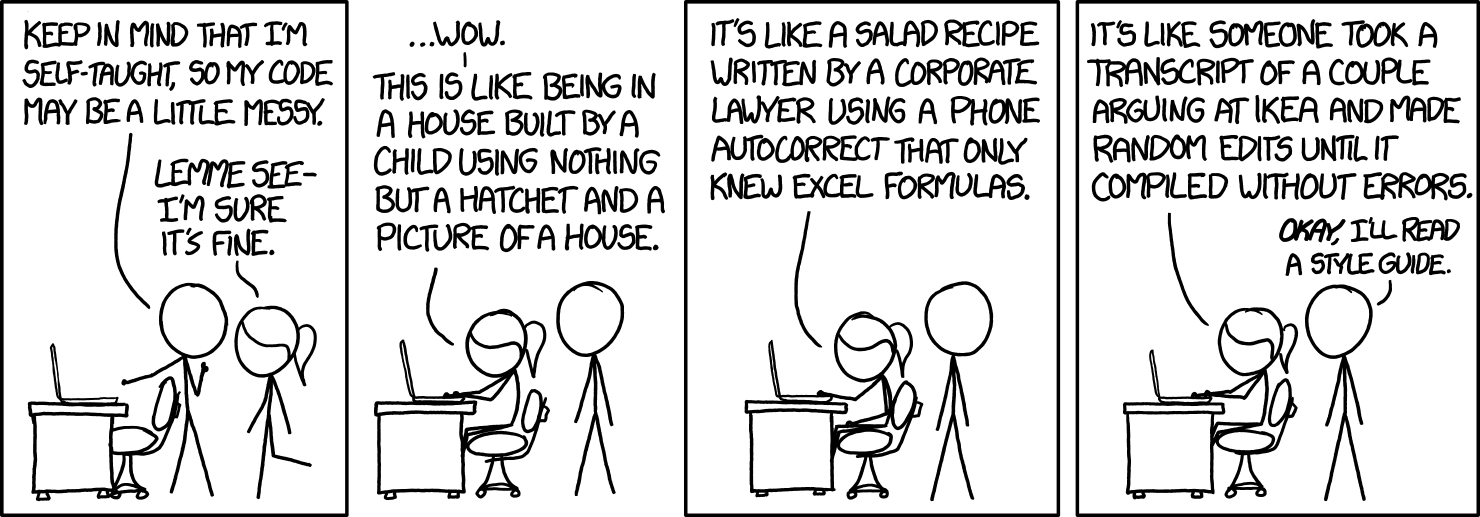
\includegraphics[width=40ex]{xkcd-reading}\\[-1ex]
		{\tiny \textcopyright~\url{https://xkcd.com/1513/}, CC BY-NC 2.5}
		\end{tabular}
		\end{center}

\end{frame}

\begin{frame}{Proof Techniques}

\begin{center}

\begin{tabular}{c}
		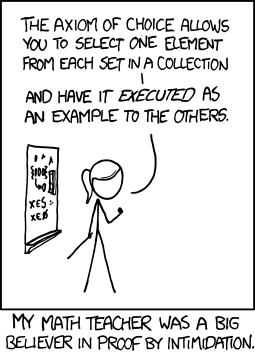
\includegraphics[width=30ex]{xkcd-proof}\\[-1ex]
		{\tiny \textcopyright~\url{https://xkcd.com/982/}, CC BY-NC 2.5}
		\end{tabular}
		\end{center}

\end{frame}

\begin{frame}{Conditional Proof}

We prove an if-then by assuming the ``if'' and deriving the ``then.''
		
		\begin{itemize}
		
		\item \textbf{Proposition}. Let $n,m$ be natural numbers. If $n$ is even, $n\cdot m$ is even.
			\item \emph{Proof}. Let $n$ and $m$ be natural numbers. We want to prove that if $n$ is even, $n\cdot m$ is even. So assume for conditional proof that $n$ is even. Then, by definition, we have that there exists a natural number $k$ such that $n=2k$. Now consider the number $n\cdot m$. Since $n=2k$, we have that $n \cdot m=(2\cdot k)\cdot m=2\cdot (k\cdot m)$. By definition, this means that $n\cdot m$ is even, which is what we wanted to show.
	
	\item \emph{How to write a conditional proof}:
			
				\begin{enumerate}[1.]
				
					\item State the conditional you wish to prove.					
					\item Assume the if-part. 
					
					\item Use mathematical reasoning to get to the then-part.
					
					\item Conclude the proof by saying that you've shown what needed to be shown.
								
				\end{enumerate}
				
		\end{itemize}

\end{frame}

\begin{frame}{Distinction by Cases}

We prove a claim by showing it in each of a list of exhaustive cases.

\begin{itemize}
	\item \textbf{Proposition}. For $n$ a natural number, $n^2+n$ is even. 
	
	\item  \emph{Proof}. Let $n$ be a natural number. First, note that $n^2+n=n(n+1)$. So it suffices to show that $n(n+1)$ is even. Since every number is either even or odd, we can distinguish two exhaustive cases: (i) $n$ is even or (ii) $n$ is odd. 
			
			\begin{itemize}
			
				\item \emph{Case i}. If $n$ is even, then $n(n+1)$ is the product of an even number, $n$, and an odd number, $n+1$. By the above proposition (the example proposition for conditional proof), this means that $n(n+1)$ is even, too.
				
				\item \emph{Case ii}. If $n$ is odd, then, by one of our previously established proposition, we know that $n+1$ is even. But then, again, $n(n+1)$ is the product of an even number, $n+1$, and an odd number, $n$, which we already observed means that $n(n+1)$ is even.
			
			\end{itemize}
			
			So, either way, $n(n+1)$ is even, which is what we wanted to show.
			
	\end{itemize}

\end{frame}

\begin{frame}{Distinction by Cases (Cont'd)}

	 \emph{How to write a proof by cases}:
			
				\begin{enumerate}[1.]
				
					\item Give a justification for your case distinction (How many cases are there? Why are they exhaustive?).
					
					\item Go through each case one by one and show, by mathematical reasoning, that the result holds in the case.
					
					\item Conclude that, since the list was exhaustive, the result holds in general.
				
				\end{enumerate}
				
		
		\begin{quote}
		There are two types of people in this world:
		
		\begin{enumerate}[1)]
		
			\item Those who can extrapolate from incomplete data.
		
		\end{enumerate}
		\begin{flushright}
		\sf{Anon}
		\end{flushright}
		
		\end{quote}

\end{frame}

\begin{frame}{Proof by Contradiction}

We prove a claim by showing that it's negation leads to a contradiction.

\begin{itemize}

\item \textbf{Proposition}. 				There is no smallest positive real number, i.e. there exists no real number $x>0$ such that for all $y>0$ we have $x\leq y$.  

\item \emph{Proof}. 				Suppose (for proof by contradiction) that our claim is false, i.e. there exists a natural number $x$ such that (i) $x>0$ and (ii) for all $y>0$ we have $x\leq y$. Call that number $\epsilon$ (as a temporary constant, cf. 2.2.8). Now consider the number $\frac{\epsilon}{2}$. Since by assumption (i) $0<\epsilon$, we have that (a) $0<\frac{\epsilon}{2}$ and that (b) $\frac{\epsilon}{2}<\epsilon$. From (a) together with (ii), it follows that $\epsilon\leq \frac{\epsilon}{2}$. But from this and (b), we get that $\epsilon<\epsilon$, which is impossible. Hence, $\epsilon$ cannot exist and our claim is proven. 

\end{itemize}

\end{frame}

\begin{frame}{Proof by Contradiction (Cont'd)}

 How to write an indirect proof:
			
				\begin{enumerate}[1.]
				
					\item State that you're assuming that the claim is false (you can note that you do this for proof by contradiction, but typically that's clear).
					
					\item Spell out what it means for the claim to be false.
					
					\item Derive a contradiction from the assumption that the claim is false.
					
					\item Conclude that the claim must be true because its negation leads to a contradiction.
									
				\end{enumerate}
				
				\begin{center}

\begin{tabular}{c}
		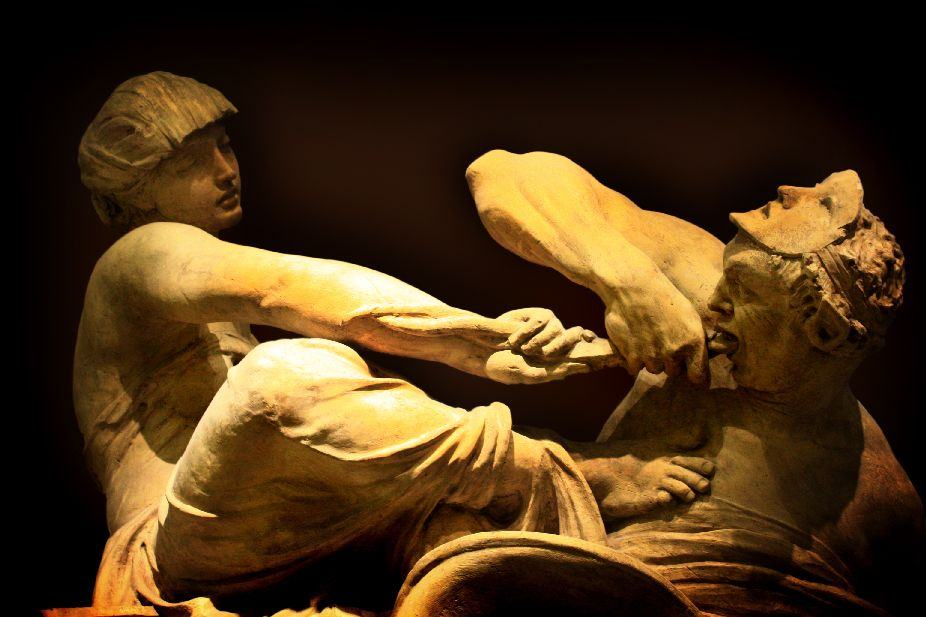
\includegraphics[width=25ex]{truth-and-falsehood}\\[-1ex]
		{\tiny \textcopyright~\texttt{Iza Bella}, \url{https://commons.wikimedia.org/wiki/File:BLW_Truth_and_Falsehood.jpg}, CC BY-SA 2.0 UK}
		\end{tabular}
		\end{center}
\end{frame}

\begin{frame}{Contrapositive Proof}

We prove an if-then by deriving ``not-if'' from ``not-then.''

\begin{itemize}

	\item \textbf{Proposition.} Let $n,m$ be natural numbers. If $n\cdot m$ is even, then either $n$ is even or $m$ is even.

	\item \emph{Proof}.				Suppose that $n$ and $m$ are natural numbers. We want to show that $n\cdot m$ is even, then either $n$ is even or $m$ is even. We prove the contrapositive, i.e. if neither $n$ nor $m$ is even, then $n\cdot m$ is odd. Note that if neither $n$ nor $m$ is even, then both $n$ and $m$ are both odd. This means that $n=2k+1$ and $m=2l+1$ for natural numbers $k,l$. Now consider the number $n\cdot m$. Since  $n=2k+1$ and $m=2l+1$, we have that $n\cdot m=(2k+1)(2l+1)=4kl+2k+2l+1=2(2kl+k+l)+1$. But now note that $2(2kl+k+l)+1$ is of the form $2x+1$ for $x$ a natural number, just let $x=2kl+k+l$. But this just means that $2(2kl+k+l)+1=n\cdot m$ is odd, which is what we needed to show.


\end{itemize}

\end{frame}

\begin{frame}{Biconditional Proof}

We show an iff by showing the if ($\Rightarrow$) and the only-if ($\Leftarrow$)

\begin{itemize}

	\item \textbf{Proposition.} A natural number $n$ is even iff $n^2$ is even.

	\item \emph{Proof}.
					
					\begin{itemize}
					
						\item ($\Rightarrow$): We need to show that if $n^2$ is even, then $n$ is even. We prove the contrapositive. Suppose that $n$ is not even, i.e. odd. Then, by previous observation, there exists a natural number $k$ such that $n=2k+1$. Now consider $n^2$. By our observation, we have $n^2=(2k+1)^2$. So, we get: $n^2=(2k+1)^2=4k^2+4k+1$. But note that $4k^2+4k=2(k^2+2k)$, and hence $4k^2+4k$ is even by definition. So $n^2=l+1$ where $l$ is an even number (just let $l=4k^2+4k$), which means that $n^2$ is odd by a previous observation. 
						
						\item ($\Leftarrow$): We want to prove that if $n$ is even, then $n^2$ is even. So suppose that $n$ is even (for conditional proof). We've previously observed that the product of an even number with any other number is even. But $n^2=n\cdot n$, so it follows as a simple corollary that $n^2$ is even.
											
					\end{itemize}

\end{itemize}

\end{frame}

\begin{frame}{Biconditional Proof (Cont'd)}

How to write a biconditional proof:
			
				\begin{enumerate}[1.]
				
					\item State that you want to prove an iff-claim.
					
					\item Prove the left-to-right direction.
					
					\item Prove the right-to-left direction.
					
					\item Conclude that the equivalence holds.
									
				\end{enumerate}
				
								\begin{center}

\begin{tabular}{c}
		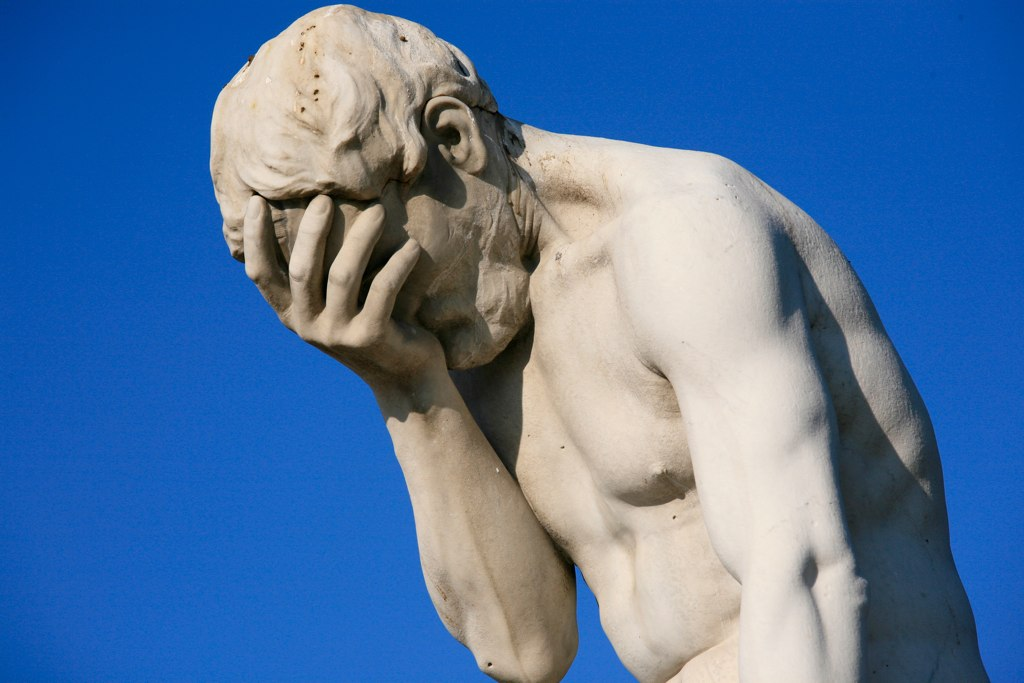
\includegraphics[width=25ex]{facepalm}\\[-1ex]
		{\tiny \textcopyright~\texttt{Alex E. Proimos}, \url{https://www.flickr.com/photos/proimos/4199675334/}, CC BY 2.0}
		\end{tabular}
		\end{center}

\end{frame}

\subsection{2.4 Some Friendly Advice}
\begin{frame}{2.4 Friendly Advice --- How to Think Like a Mathematician}

Advice from Kevin Houston (HTTLAM, p.~x):
	
	\begin{itemize}
		
			\item \emph{It’s up to you}
			
			\item  \emph{Be active}

			\item  \emph{Think for yourself}
			
			\item  \emph{Question everything} 
			
			\item  \emph{Observe} 
			
			\item  \emph{Prepare to be wrong}

			\item  \emph{Don't memorize} (seek to understand)
			
			\item  \emph{Develop your intuition}
			
			\item  \emph{Collaborate}
						
			\item  \emph{Reflect} 
			
		\end{itemize}
	

\end{frame}


\begin{frame}{Core Ideas (Lecture Version)}
	
\begin{itemize}

		\item You have to learn mathemateze like a foreign language

		\item Variables stand for arbitrary but fixed objects, constants stand for known objects. 

		\item An object is defined by giving a list of properties that the object and only the object satisfies. We need to prove existence and uniqueness. 	
				
		\item A property or relation is defined by giving the conditions for an object has the property or some objects stand in the relation. It mustn't be circular.
		
		\item  A mathematical proof is a rigorous, step-by-step argument which establishes the truth of a mathematical statement. 


		\item Think of proving as problem solving. 
		
		\item Follow the advice!

	\end{itemize}


\end{frame}

\begin{frame}

	\begin{center}
	{\huge\bf Thanks!}
	\end{center}

\end{frame}

